\section{Analysis}

\subsection{Stake Holders}
    This project is designed with computer science education in mind. As such potential stake holders could include various educational institutions as well as individual teachers and tutors. For example, the project could be used in a sixth-form or university classroom to demonstrate the workings of the x86 architecture or the more general workings of a typical Von Neumann architecture CPU.

\subsection{Computational Methods}
    A computational solution is appropriate here for a number of reasons. One such reason is that one of the best ways for potential stake holders (i.e. teachers) to teach about the low-level workings of an x86 system is show some such system in action. While theoretically they could indeed source an old IBM PC or similar for this purpose, doing so nowadays is rather difficult and expensive due to the rarity of such old systems. Instead, a simpler alternative is to just run emulators of these old systems using their existing modern hardware. Another bonus of doing this as an alternative is that an emulator allows for far more precise information about and control of the running of the system. Indeed, this is a key aspect that I think will allow my project specifically to be useful in the domain of education as a key focus of its design is allowing for the exposure of the inner workings of the emulated system.

    \subsubsection{Abstraction}
        A far degree of computational abstraction can be seem throughout the project's codebase.

    \subsubsection{Decomposition}
        The basic running of the emulator itself (excluding GUI interactions) can be broken down into the following:
        \begin{itemize}
            \item Load
        \end{itemize}

        See figure \ref{fig:...} below for a detailed breakdown of the components this project is comprised of. This was achieved using the divide \& conquer method of decomposition.

        \begin{figure}[h]
            \centering
            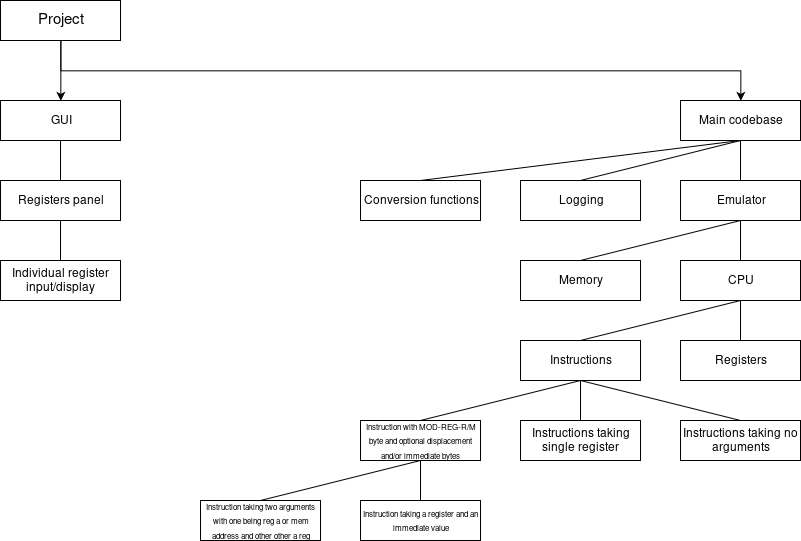
\includegraphics{decomposition}
            \caption{Decomposition of the project.}
            \label{fig:...}
        \end{figure}

\subsection{Features \& Limitations}
    One feature that was required as part of the coursework specification was a Graphical User Interface (GUI). The choice of GUI library to use proved to be more challenging than anticipated - see section \ref{...} of the Design portion of this document for more information.

    As stated above, one key feature of the emulator should be its applicability to a teaching environment. As such, detailed information regarding the running of the emulator (state of registers, assembly expression of the current instruction, state of main memory, etc.) should be readily available. In addition, ability to modify the state of emulator should be possible to allow students to learn through the consequences of any modifications they make. On the topic of modification, the source code of the project must be well organised, cleanly written, and fully documented so that students may learn through reading its implementation and by potentially making modifications to the software itself.

    Speed of execution is most certainly not to be prioritised during development meaning any optimisations that could be made to the code at the expense of readability or stability are not to be made. This lack of optimisation could potentially be presented as a limitation of the software in certain situations. However, due to emulation of such old hardware not being particularly resource-intensive as well as the project being implemented in the fast, compiled C++ language, this should not present any significant issues.

\subsection{Requirements} % requirements for development to happen, requirements of stackholders.

\subsection{Existing Projects}
    There are a few different existing emulators of the Intel 8086 microprocessor and associated hardware.

\subsection{Success Criteria}
    The original success criteria of this project was far too ambitious given the limited time available to be dedicated to this project. Originally, it was planned that the emulator would be considered complete only once it was capable of running a Basic Input Output System (BIOS) and then successfully booting an early version of Microsoft Disk Operating System (MS-DOS). While this of course would have been rather impressive, it would have required an entirely bug-free implementation of the entirety of the Intel 8086, Intel 8259 Programmable Interrupt Controller, Intel 8253 Programmable Interval Timer, etc.
